%
%

%%-----------------------------------------------------
%%-----------------------------------------------------
\section{El alfabeto de la élite}

%%-----------------------------------------------------
\begin{frame}
\frametitle{Leetspeak}

\begin{columns}[T]
\begin{column}{.48\textwidth}

  {\Huge
    ¿s4b35 h4bl4r \\
    c0m0 l05 fr1k15 \\
    d3 v3rd4d? \\
  }
  \vspace{1cm}
\begin{flushright}
  {
    \url{https://en.wikipedia.org/wiki/Leet}
  }
\end{flushright}

\end{column}%
\hfill%
\begin{column}{.50\textwidth}
{\Large
\begin{itemize}
\item Leet (``1337'') es un alfabeto alternativo
\item Origen: BBSs de los años 1980
\item ``El habla de la élite'' (admin de las BBS)
\item Muchas variantes
\item Incluye vocabuliario, gramática...
\item Ejemplo: ``31337 h4x0r''
\end{itemize}
}
\end{column}%
\end{columns}

\end{frame}

%%-----------------------------------------------------
\begin{frame}
\frametitle{Hay conversores...}

\begin{center}
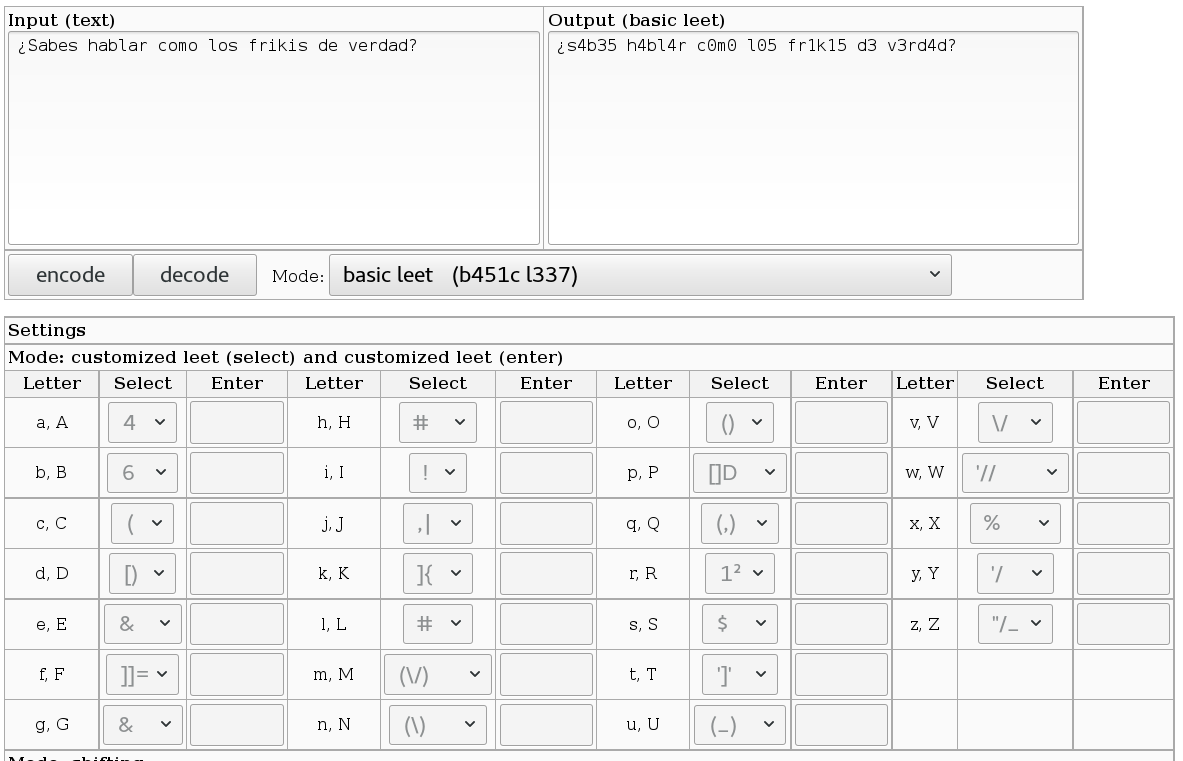
\includegraphics[height=6.5cm]{figs/leetspeak-converter}
\end{center}

\begin{flushright}
  \url{http://www.robertecker.com/hp/research/leet-converter.php}
\end{flushright}

\end{frame}

%%-----------------------------------------------------
\begin{frame}[fragile]
\frametitle{Geek code}

{\Large
\begin{verbatim}
-----BEGIN GEEK CODE BLOCK-----
GED/J d-- s:++>: a--
C++(++++) ULU++ P+ L++
E---- W+(-) N+++ o+ K+++ w--- O-
M+ V--
PS++>$ PE++>$
Y++ PGP++ t-
5+++ X++ R+++>$
TV+ b+ DI+++ D+++ G+++++ e++  h r--
y++**
------END GEEK CODE BLOCK------
\end{verbatim}
}

\begin{flushright}
  \url{https://en.wikipedia.org/wiki/Geek_Code}
\end{flushright}

\end{frame}






